\documentclass{beamer}
\usepackage{beamerthemesplit}
\usepackage{booktabs}
\RequirePackage{graphicx}
\RequirePackage[italian]{babel}
\usepackage[utf8x]{inputenc}


\title[]{Linked Open Data per la realizzazione di un Content-based Recommender System}
\institute{ \textbf{Accesso intelligente alle informazioni ed \\ elaborazione del linguaggio naturale\\}
~ \\
\begin{small}
Corso di Laurea in Informatica Magistrale
\end{small}}
\author{\textbf{Luciano Quercia}\\
\textbf{Simone Rutigliano}}
\date{\tiny{\today}}


%\usetheme{Hannover}
\usetheme{Copenhagen}
\usecolortheme{seahorse}
\usecolortheme{rose}
%\usetheme{Frankfurt}
%\usecolortheme{beetle}

%\useoutertheme[subsection=false]{smoothbars}
%\useoutertheme[subsection=false]{smoothtree}
\useoutertheme{shadow}
\setbeamercovered{dynamic}

\pgfdeclareimage[height=1cm]{logo}{figure/logo}
\logo{\pgfuseimage{logo}}


\begin{document}

\begin{frame}
\maketitle
\end{frame}

\section{Obiettivi}

\subsection{Classificatore}
\begin{frame}
\frametitle{TEPaC}
TEPaC

\emph{Transductive Emerging Pattern based Classifier}

\begin{itemize}
\item classificatore di strutture logiche
\item basato su pattern emergenti
\item utilizza un approccio trasduttivo
\end{itemize}

\end{frame}

%%%%%%%%%%%%%%%%%%%%%%%%%%%%%%%%%%%%%%%%%%%
%%%%%%%%%%%%%%%%%%%%%%%%%%%%%%%%%%%%%%%%%%%
%%%%%%%%%%%%%%%%%%%%%%%%%%%%%%%%%%%%%%%%%%%

\subsection{Document Image Understanding}
\begin{frame}
\frametitle{Document Image Understanding}

\begin{columns}
\begin{column}{0.6\textwidth}

\begin{itemize}
\item<1-> Comprensione automatizzata di documenti cartacei
\item<2-> La maggior parte della conoscenza mondiale si trova su supporti cartacei
\begin{itemize}
\item Libri
\item Documenti
\item Giornali
\end{itemize}
\item<3-> La digitalizzazione offre innumerevoli vantaggi
\end{itemize}
\end{column}

\begin{column}{0.2\textwidth}
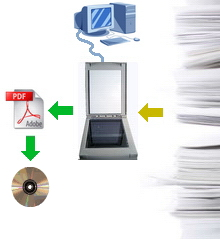
\includegraphics[width=3cm]{figure/diu.jpg}
\end{column}

\end{columns}

\end{frame}


%%%%%%%%%%%%%%%%%%%%%%%%%%%%%%%%%%%%%%%%%%%
%%%%%%%%%%%%%%%%%%%%%%%%%%%%%%%%%%%%%%%%%%%
%%%%%%%%%%%%%%%%%%%%%%%%%%%%%%%%%%%%%%%%%%%


\begin{frame}
\begin{scriptsize}

\begin{columns}
\begin{column}{0.4\textwidth}
	\begin{tabular}{c | ccc}
	\toprule
	 & \multicolumn{3}{c}{$minSup\ (\%)$} \\
	$minGR$ & 30 & 40 & 50 \\
	\hline
	1  & 528032 & 344798 & 254805 \\
	2  & 523274 & 341534 & 252355 \\
	8  & 516958 & 336733 & 248658 \\
	64 & 513503 & 334292 & 246843 \\
	\bottomrule
	\end{tabular}
Dataset TPAMI
	\vspace{8 mm}
	
	\begin{tabular}{c | ccc}
	\toprule
	 & \multicolumn{3}{c}{$minSup\ (\%)$} \\
	$minGR$ & 10 & 20 & 30 \\
	\hline
	1  & 386996 & 176407 & 114492 \\
	2  & 382639 & 173372 & 112476 \\
	8  & 376645 & 169406 & 109814 \\
	64 & 374736 & 167742 & 108595 \\
	\bottomrule
	\end{tabular}
Dataset ICML

\end{column}

\begin{column}{0.4\textwidth}
	\begin{tabular}{c | ccc}
	\toprule
	 & \multicolumn{3}{c}{$minSup\ \ (\%)$} \\
	$minGR$ & 10 & 20 & 30 \\
	\hline
	1  & 128327 & 88684 & 58603 \\
	2  & 126840 & 87644 & 58091 \\
	8  & 122591 & 84208 & 55718 \\
	64 & 121363 & 82980 & 54490 \\
	\bottomrule
	\end{tabular}
Dataset BG

\end{column}
\end{columns}

\end{scriptsize}
\end{frame}


\begin{frame}
\begin{center}
Grazie per l'attenzione.
\end{center}
\end{frame}
\end{document}
